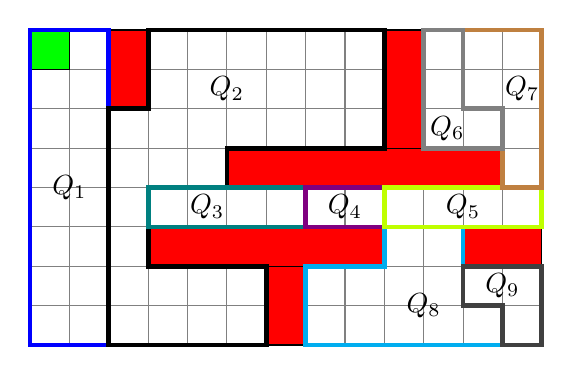
\begin{tikzpicture}[scale=1]
\draw[step=0.5cm,color=gray] (-3.5,-2) grid (3,2);


\filldraw[fill=green,draw=black] (-3.5,2) rectangle (-3,1.5);
% \filldraw[fill=red,draw=black] (-2.5,2) rectangle (-2,1.5);
\filldraw[fill=red,draw=black] (-2.5,2) rectangle (-2,1.0);
\filldraw[fill=red,draw=black] (1,2) rectangle (1.5,0.0);
\filldraw[fill=red,draw=black] (-1,0.5) rectangle (2.5,0.0);
\filldraw[fill=red,draw=black] (2,-0.5) rectangle (3,-1.0);
\filldraw[fill=red,draw=black] (-2,-0.5) rectangle (1,-1.0);
\filldraw[fill=red,draw=black] (-0.5,-1.0) rectangle (0,-2.0);

\filldraw[fill=none,draw=blue,line width=0.6mm] (-3.5,2.0) rectangle (-2.5,-2.0);
\draw[black, line width = 0.6mm] plot coordinates{(-2.0,2) (-2.0,1) (-2.5,1) (-2.5,-2) (-0.5,-2) (-0.5,-1) (-2.0,-1) (-2.0,-0.0) (-1.0,-0.0) (-1.0,0.5) (1.0,0.5) (1.0,2)}--cycle;
\draw[cyan, line width = 0.6mm] plot coordinates{(0,-1.0) (0,-2.0) (3,-2.0) (3,-1.0) (2,-1.0) (2,-0.5) (1,-0.5) (1,-1.0)}--cycle;


\filldraw[fill=none,draw=teal, line width=0.6mm] (-2.0,0.0) rectangle (-0.0,-0.5);
\filldraw[fill=none,draw=violet, line width=0.6mm] (-0.0,0.0) rectangle (1.0,-0.5);
\filldraw[fill=none,draw=lime, line width=0.6mm] (1.0,0.0) rectangle (3.0,-0.5);
\draw[brown, line width = 0.6mm] plot coordinates{(2.0,2.0) (2.0,1.0) (2.5,1.0) (2.5,0.0) (3.0,0.0) (3.0,2.0)}--cycle;
\draw[gray, line width = 0.6mm] plot coordinates{(1.5,2.0) (1.5,0.5) (2.5,0.5) (2.5,1.0) (2.0,1.0) (2.0,2.0)}--cycle;
\draw[darkgray, line width = 0.6mm] plot coordinates{(2.0,-1.0) (2.0,-1.5) (2.5,-1.5) (2.5,-2.0) (3,-2.0) (3,-1)}--cycle;


% \filldraw[fill=blue!40!white,draw=black] (+0.75,+0.75) circle (0.2cm);
% \filldraw[fill=orange!40!white,draw=black] (0.25,-0.75) circle (0.2cm);
\node at (-3.0,+0.0) {\textbf{$Q_1$}};
\node at (-1.25,-0.25) {\normalsize{\textbf{$Q_3$}}};
\node at (-1.0,1.25) {\normalsize{\textbf{$Q_2$}}};
\node at (1.5,-1.5) {\normalsize{\textbf{$Q_8$}}};
\node at (0.5,-0.25) {\normalsize{\textbf{$Q_4$}}};
\node at (2.0,-0.25) {\normalsize{\textbf{$Q_5$}}};
\node at (1.8,0.75) {\normalsize{\textbf{$Q_6$}}};
\node at (2.75,1.25) {\normalsize{\textbf{$Q_7$}}};
\node at (2.5,-1.25) {\normalsize{\textbf{$Q_9$}}};
% \node at (-1.5,-0.0) {\large{\textbf{2}}};
% \node at (-0.30,+0.75) {\tiny{2}};
% \node at (0.20,+0.75) {\tiny{3}};
% \node at (0.73,+0.75) {\tiny{4}};
% \node at (-1.33,+0.25) {\tiny{5}};
% \node at (-0.85,+0.25) {\tiny{6}};
% \node at (-0.35,+0.25) {\tiny{7}};
% \node at (0.25,+0.25) {\tiny{8}};
% \node at (0.75,+0.25) {\tiny{9}};
% \node at (-1.28,-0.27) {\tiny{10}};
% \node at (-0.78,-0.27) {\tiny{11}};
% \node at (-0.28,-0.27) {\tiny{12}};
% \node at (0.28,-0.27) {\tiny{13}};
% \node at (0.75,-0.25) {\tiny{14}};
% \node at (-1.3,-0.75) {\tiny{15}};
% \node at (-0.8,-0.75) {\tiny{16}};
% \node at (-0.3,-0.75) {\tiny{17}};
% \node at (0.25,-0.75) {\tiny{18}};
% \node at (0.75,-0.75) {\tiny{19}};
% \node at (-1.27,-1.25) {\tiny{20}};
% \node at (-0.8,-1.25) {\tiny{21}};
% \node at (-0.3,-1.25) {\tiny{22}};
% \node at (0.25,-1.25) {\tiny{23}};
% \node at (0.75,-1.25) {\tiny{24}};
\end{tikzpicture}